\documentclass[11pt]{article}
\usepackage[a4paper, margin=2.54cm]{geometry}
\usepackage[utf8]{inputenc}
\usepackage[spanish, mexico]{babel}
\usepackage[spanish]{layout}
\usepackage[article]{ragged2e}
\usepackage{textcomp}
\usepackage{amsmath}
\usepackage{amssymb}
\usepackage{amsfonts}
\usepackage{graphicx}
\usepackage{array}
\usepackage{multirow}
\usepackage{enumerate}

\setlength{\parindent}{5pt}

\title{
    Trabajo Práctico IPv6 \\
    \large Comunicaciones}
\author{Mellino, Natalia \and Farizano, Juan Ignacio}
\date{}

\begin{document}
\maketitle
\noindent\rule{\textwidth}{1pt}


\section{Objetivo: analizar aspectos de IPv6 sobre una PC y sobre un enlace de PCs.}

\subsection*{Apartado c)}

Revisamos la configuración de IP de Windows.

\begin{verbatim}
  C:\Users\Fari>ipconfig

  Windows IP Configuration
  
  Ethernet adapter Ethernet:
  
     Media State . . . . . . . . . . . : Media disconnected
     Connection-specific DNS Suffix  . :
  
  Wireless LAN adapter Wi-Fi:
  
     Connection-specific DNS Suffix  . : fibertel.com.ar
     Link-local IPv6 Address . . . . . : fe80::8d23:e573:afc7:a088%15
     IPv4 Address. . . . . . . . . . . : 192.168.0.222
     Subnet Mask . . . . . . . . . . . : 255.255.255.0
     Default Gateway . . . . . . . . . : 192.168.0.1  
\end{verbatim}

\subsection*{Apartado d)}

Realizamos ping hacia el propio equipo (loopback o ::1).

\begin{verbatim}
    C:\Users\Fari>ping ::1

    Pinging ::1 with 32 bytes of data:
    Reply from ::1: time<1ms
    Reply from ::1: time<1ms
    Reply from ::1: time<1ms
    Reply from ::1: time<1ms

    Ping statistics for ::1:
        Packets: Sent = 4, Received = 4, Lost = 0 (0% loss),
    Approximate round trip times in milli-seconds:
        Minimum = 0ms, Maximum = 0ms, Average = 0ms
\end{verbatim}

\subsection*{Apartado e)}

Realizamos ping desde una notebook hacia la PC que está capturando paquetes
con Wireshark.

\begin{verbatim}
  C:\Users\Fari> ping fe80::5252:517c:8dd7:2323

  Pinging fe80::5252:517c:8dd7:2323 with 32 bytes of data:
  Reply from fe80::5252:517c:8dd7:2323: time=5ms
  Reply from fe80::5252:517c:8dd7:2323: time=2ms
  Reply from fe80::5252:517c:8dd7:2323: time=2ms
  Reply from fe80::5252:517c:8dd7:2323: time=2ms
  
  Ping statistics for fe80::5252:517c:8dd7:2323:
      Packets: Sent = 4, Received = 4, Lost = 0 (0% loss),
  Approximate round trip times in milli-seconds:
      Minimum = 2ms, Maximum = 5ms, Average = 2ms
\end{verbatim}

\subsection*{Apartado f)}
Tomamos uno de los paquetes capturados con Wireshark y analizamos su cabecera:

\begin{verbatim}
  0110 .... = Version: 6
  .... 0000 0000 .... .... .... .... .... = Traffic Class: 0x00 (DSCP: CS0, ECN: Not-ECT)
  .... .... .... 0000 0000 0000 0000 0000 = Flow Label: 0x00000
  Payload Length: 40
  Next Header: ICMPv6 (58)
  Hop Limit: 128
  Source: fe80::8d23:e573:afc7:a088
  Destination: fe80::5252:517c:8dd7:2323
\end{verbatim}

Observamos que en la cabecera aparecen los campos: Versión de Protocolo, indicando que estamos 
utilizando IPv6; luego, tenemos la Clase de Tráfico, Etiqueta de flujo, Longitud del Paquete,
Siguiente Cabecera (indicando que la misma es ICMPv6), el límite de saltos, que es el Time
To Live del paquete, y por último las direcciones IP de origen y destino en Source y Destination
respectivamente. 

\subsection*{Apartado g)}

Pudimos observar que se dio el proceso de Neighbor Discovery antes de realizar
el ping mediante la captura de los siguientes paquetes:

\begin{verbatim}
# Info. del primer paquete
Source: fe80::8d23:e573:afc7:a088
Destination: ff02::1:ffd7:2323
Protocol: ICMPv6
Info: Neighbor Solicitation for fe80::5252:517c:8dd7:2323 from 70:c9:4e:da:8b:37

# Info. del segundo paquete
Source: fe80::5252:517c:8dd7:2323
Destination: fe80::8d23:e573:afc7:a088
Protocol: ICMPv6
Info: Neighbor Advertisement fe80::5252:517c:8dd7:2323 (sol, ovr) is at 04:d9:f5:04:99:e2
\end{verbatim}

Se puede ver que el primer dispositivo (la notebook), envía un paquete ICMPv6
con el tipo de mensaje Neighbor Solicitation a una dirección Multicast solicited-node
asociada a la computadora destino. Y esta responde con otro paquete ICMPv6 con el
tipo de mensaje Neighbor Advertisement que contiene su dirección MAC.

\section{Objetivo: utilizar una red simulada, visualizando Router Discovery y/o descubrimiento de vecinos}

\subsection*{Tarea 2}

\subsubsection*{Apartado b)}

\begin{tabular}{|c c|c|c|c|}
  \hline
   \multicolumn{2}{|c|}{\multirow{2}{*}{\textbf{Dispositivo}}} & 
   \multirow{2}{2cm}{\centering\textbf{IPv6 \\ habilitado}} & 
   \multirow{2}{2cm}{\centering\textbf{Dirección IP Local}} & 
   \multirow{2}{2cm}{\centering\textbf{Dirección IP Global}} \\ 
   & & & & \\ \hline
   \multirow{2}{*}{Routers0} & Fa0/0 & Sí & FE80::2D0:D3FF:FEB4:1301 & 2001:DB8:1:0:2D0:D3FF:FEB4:1301 \\
                             & Fa0/1 & Sí & FE80::2D0:D3FF:FEB4:1302 & 2001:DB8:2:0:2D0:D3FF:FEB4:1302 \\ \hline
   \multirow{2}{*}{Routers1} & Fa0/0 & Sí & FE80::205:5EFF:FE41:601 & 2001:DB8:3:0:205:5EFF:FE41:601 \\
                             & Fa0/1 & Sí & FE80::205:5EFF:FE41:602 & 2001:DB8:2:0:205:5EFF:FE41:602 \\ \hline
\end{tabular}

\begin{enumerate}[a)]
  \item Una dirección IPv6 tiene 128 bits.
  \item El prefijo asignado por el RIR es 2001:DB8:1::/64, como la máscara es de 64
        bits, no tiene subred. El ID de interfaz es: 2D0:D3FF:FEB4:1301.
  \item La dirección de la MAC es: 00D0.D3B4.1301, a partir de ella podemos
        construir la dirección IPv6 Link-Local de la interfaz siguiendo estos pasos:
        \begin{enumerate}[1)]
          \item Dividimos la dirección en 2 y en el medio agregamos el valor hexadecimal FFFE \\
                00D0.D3 FFFE B4.1031
          \item En el primer octeto invertimos el índice número 6, lo convertimos a hexadecimal
                y utilizamos la notación de IPv6. \\
                Con esto ya tenemos nuestra interface ID: 02D0:D3FF:FEB4:1031
          \item Por último, agregamos el prefijo FE80 y ya tenemos nuestra dirección IPv6 Link-Local. \\
                FE80::2D0:D3FF:FEB4:1301       
        \end{enumerate}
  \item 
    \begin{verbatim}
      # Tabla de ruteo del router0
      Router>show ipv6 route
      IPv6 Routing Table - 6 entries
      Codes: C - Connected, L - Local, S - Static, R - RIP, B - BGP
             U - Per-user Static route, M - MIPv6
             I1 - ISIS L1, I2 - ISIS L2, IA - ISIS interarea, IS - ISIS summary
             ND - ND Default, NDp - ND Prefix, DCE - Destination, NDr - Redirect
             O - OSPF intra, OI - OSPF inter, OE1 - OSPF ext 1, OE2 - OSPF ext 2
             ON1 - OSPF NSSA ext 1, ON2 - OSPF NSSA ext 2
             D - EIGRP, EX - EIGRP external
      C   2001:DB8:1::/64 [0/0]
           via ::, FastEthernet0/0
      L   2001:DB8:1:0:2D0:D3FF:FEB4:1301/128 [0/0]
           via ::, FastEthernet0/0
      C   2001:DB8:2::/64 [0/0]
           via ::, FastEthernet0/1
      L   2001:DB8:2:0:2D0:D3FF:FEB4:1302/128 [0/0]
           via ::, FastEthernet0/1
      R   2001:DB8:3::/64 [120/2]
           via FE80::205:5EFF:FE41:602, FastEthernet0/1
      L   FF00::/8 [0/0]
           via ::, Null0

      # Tabla de ruteo del router1
      Router>show ipv6 route
      IPv6 Routing Table - 6 entries
      Codes: C - Connected, L - Local, S - Static, R - RIP, B - BGP
             U - Per-user Static route, M - MIPv6
             I1 - ISIS L1, I2 - ISIS L2, IA - ISIS interarea, IS - ISIS summary
             ND - ND Default, NDp - ND Prefix, DCE - Destination, NDr - Redirect
             O - OSPF intra, OI - OSPF inter, OE1 - OSPF ext 1, OE2 - OSPF ext 2
             ON1 - OSPF NSSA ext 1, ON2 - OSPF NSSA ext 2
             D - EIGRP, EX - EIGRP external
      R   2001:DB8:1::/64 [120/2]
           via FE80::2D0:D3FF:FEB4:1302, FastEthernet0/1
      C   2001:DB8:2::/64 [0/0]
           via ::, FastEthernet0/1
      L   2001:DB8:2:0:205:5EFF:FE41:602/128 [0/0]
           via ::, FastEthernet0/1
      C   2001:DB8:3::/64 [0/0]
           via ::, FastEthernet0/0
      L   2001:DB8:3:0:205:5EFF:FE41:601/128 [0/0]
           via ::, FastEthernet0/0
      L   FF00::/8 [0/0]
           via ::, Null0
    \end{verbatim}

    \item 
    \begin{verbatim}
      C:\>ping 2001:DB8:3:0:201:C9FF:FE63:5AEB

      Pinging 2001:DB8:3:0:201:C9FF:FE63:5AEB with 32 bytes of data:

      Reply from 2001:DB8:3:0:201:C9FF:FE63:5AEB: bytes=32 time<1ms TTL=126
      Reply from 2001:DB8:3:0:201:C9FF:FE63:5AEB: bytes=32 time<1ms TTL=126
      Reply from 2001:DB8:3:0:201:C9FF:FE63:5AEB: bytes=32 time<1ms TTL=126
      Reply from 2001:DB8:3:0:201:C9FF:FE63:5AEB: bytes=32 time<1ms TTL=126

      Ping statistics for 2001:DB8:3:0:201:C9FF:FE63:5AEB:
          Packets: Sent = 4, Received = 4, Lost = 0 (0% loss),
      Approximate round trip times in milli-seconds:
          Minimum = 0ms, Maximum = 0ms, Average = 0ms
    \end{verbatim}
  \end{enumerate}

\newpage

\subsection*{Tarea 4}

\subsubsection*{Apartado d)}

\begin{figure}[h!]
  \begin{center}
    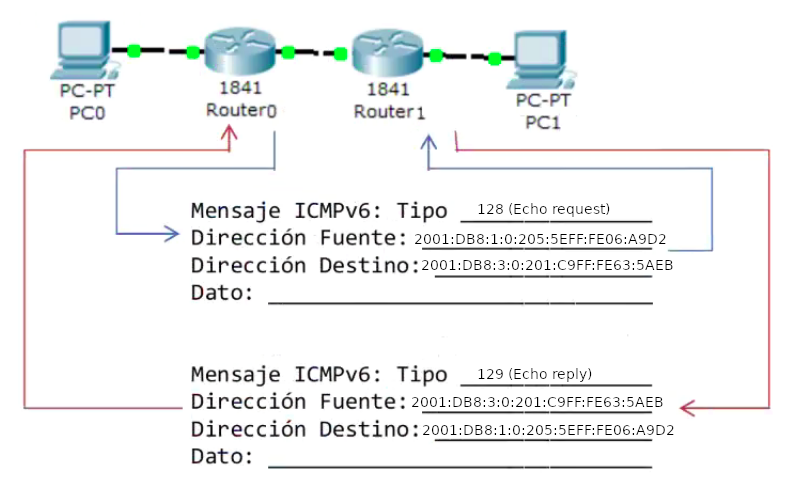
\includegraphics[width=0.95\linewidth]{4d.png}
  \end{center}
\end{figure}

\subsubsection*{Apartado f)}

\begin{figure}[h!]
  \begin{center}
    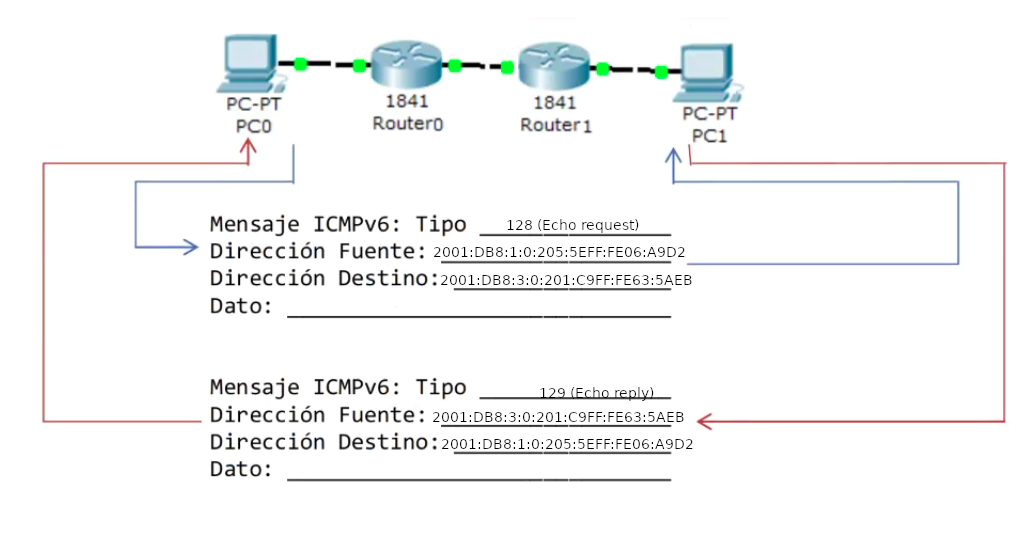
\includegraphics[width=0.95\linewidth]{4f.png}
  \end{center}
\end{figure}

\end{document}

